\chapter{RNNs and LSTMs}

\section{Vanishing and Exploding Gradients}
Training neural networks using backpropagation requires us to compute the 
partial derivatives of the loss function wrt each weight and bias of the network.
The weights and biases are then revised using these partial derivatives using the 
stochastic gradient descent formulation:
\[
    w^{\text{new}} = w^{\text{old}} - \eta \frac{\partial L}{\partial w}.
\]

If the network is deep enough, then in certain cases it possible for 
the term $\partial L / \partial w$ to be very small or very large. If this term 
is very small, then the weight is not updated; if it is very large, there is a 
large update to the weight, which keeps on repeating at each updation step, with 
the result that the weights do not converge. 

To illustrate this problem, consider a simple network with $L$ layers, with 
two neurons in each of the first $L - 1$ layers and a single neuron in the 
final layer~$L$. This network is a map from $\R^2 \to \R^1$. Let 
$W^{(i)}$ be the weight matrix associated with layer~$i$, where 
$W^{(1)}, \ldots, W^{(L - 1)} \in \R^{2 \times 2}$ and $W^{(L)} \in \R^{1 \times 2}$. 
Ignore the biases and assume that there are no activation functions. Consider 
a single input-output pair $((x_1, x_2)^{T}, y)$. 
Denote the input to layer~$i$ as $\vect{x}^{(i - 1)}$, so that input to the 
very first layer is $\vect{x}^{(0)} = (x_1, x_2)^{T}$. Then the output of 
layer~$i$, ignoring the bias and the activation, is $W^{(i)} \vect{x}^{(i - 1)}$. 
The output of the first layer is $W^{(1)} \vect{x}^{(0)}$, that of the second 
is $W^{(2)} W^{(1)} \vect{x}^{(0)}$ and so on. The final output~$\hat{y}$ of the 
network is easily seen to be:
\[
    \hat{y} = W^{(L)} \cdot W^{(L - 1)} \cdots W^{(1)} \cdot \vect{x}^{(0)}.
\]

To write this final output more explicitly in terms of the individual weights, 
we need a little more notation. Let $W^{(i)}$, for $1 \leq i \leq L - 1$, be:
\[
    \left ( 
        \begin{array}{cc}
            w_{11}^{(i)} & 0            \\
            0            & w_{22}^{(i)}
        \end{array}
    \right ).
\]
Let $W^{(L)} = (w_{11}^{(L)}, w_{12}^{(L)})$. Then 
\[\arraycolsep=1.2pt\def\arraystretch{1.9}
    \hat{y} = (w_{11}^{(L)}, w_{12}^{(L)}) \cdot 
             \left ( 
                \begin{array}{cc}
                    w_{11}^{(L - 1)} w_{11}^{(L - 2)} \cdots w_{11}^{(2)} w_{11}^{(1)} x_1 \\ 
                    w_{22}^{(L - 1)} w_{22}^{(L - 2)} \cdots w_{11}^{(2)} w_{22}^{(1)} x_2
                \end{array}
            \right ).
\]
This ultimately yields:
\[
    \hat{y} =  w_{11}^{(L)} w_{11}^{(L - 1)} w_{11}^{(L - 2)} \cdots w_{11}^{(2)} w_{11}^{(1)} x_1 
               + w_{12}^{(L)} w_{22}^{(L - 1)} w_{22}^{(L - 2)} \cdots w_{11}^{(2)} w_{22}^{(1)} x_2.
\]

Assume that the loss function is the standard squared loss: $L(y, \hat{y}) = 0.5 \cdot (y - \hat{y})^2$. 
Consider the derivative of~$L$ wrt one of the weights in the very first layer. 
\begin{align*}
    \frac{\partial L}{\partial w_{11}^{(1)}} & = 
        \frac{\partial L}{\partial \hat{y}}
        \frac{\partial \hat{y}}{\partial w_{11}^{(1)}} \\
        & = (\hat{y} - y) \cdot w_{11}^{(L)} w_{11}^{(L - 1)} \cdots w_{11}^{(2)} x_1. 
\end{align*}
Notice that the partial derivative is a product that tacks on weights, one from each 
layer, starting with the second layer. Now if $L$ is large and these weights were 
all slightly less than $1$, then resulting product would be very small; if these weights 
are slightly larger than $1$, then the product would be a large quantity. The first 
case is the \emph{vanishing gradient} problem; the second is the 
\emph{exploding gradient} problem. Note that is does not matter which 
weight we use to differentiate the loss function. The partial derivative product 
term picks up weights form each layer (except the one wrt which we are differentiating). 
 
\begin{exercise}
Can we avoid the vanishing gradient problem by using a different activation function 
than the sigmoid function?
\end{exercise}
\begin{solution}
If we use an activation function~$f$ whose derivative is higher at $f'(0)$ is higher, but
less than $1$, we can reduce the severity of the vanishing gradient problem, but not eliminate 
it altogether. If we were choose $f$ such that $f'(0) > 1$, then we might end up with the 
exploding gradient problem. 

One such candidiate function is the hyperbolic tangent function. This is defined as:
\[
    \tanh (x) = \frac{e^x - e^{-x}}{e^x + e^{-x}}.
\]
The derivative of this function is $\tanh ' (x) = 1 - \tanh (x)^2$. The graph of the 
function and its derivative is shown in Figure~\ref{fig:tanh}.

\begin{figure}[ht]
\begin{center}
\begin{minipage}[b]{0.4\textwidth}
\begin{center}
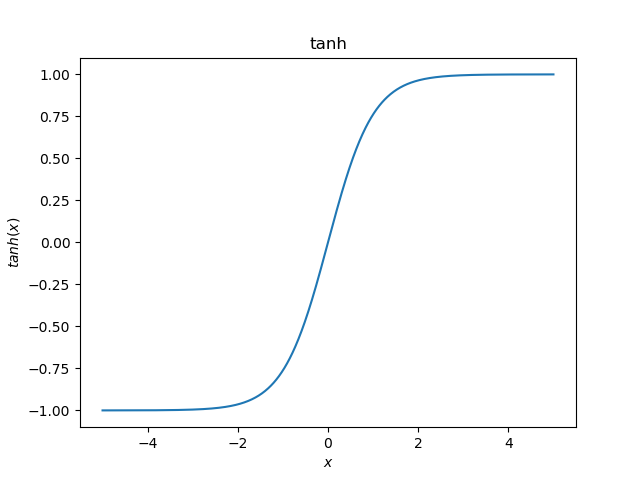
\includegraphics[width=\textwidth]{Tanh.png}
\end{center}
\end{minipage}
\begin{minipage}[b]{0.4\textwidth}
\begin{center}
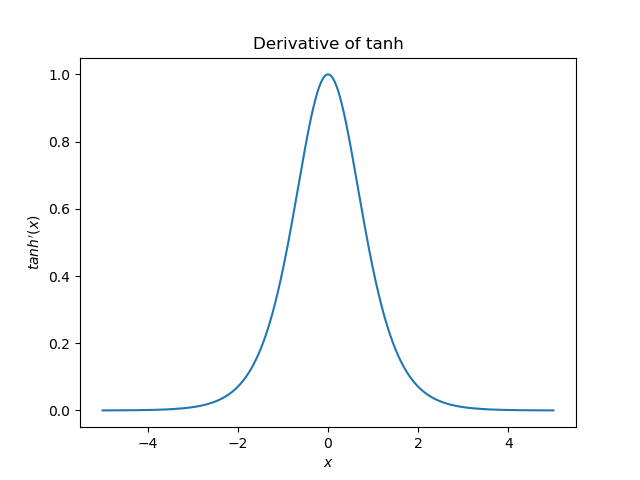
\includegraphics[width=\textwidth]{TanhDerivative.png}
\end{center}
\end{minipage}
\caption{The Tanh function and its derivative}
\label{fig:tanh}
\end{center}
\end{figure}
\end{solution}
\section{LSTMs}
These notes are based on~\cite{EChen,COlah}. LSTMs were developed in order to
circumvent the vanishing gradient problem that
plagues multi-layered RNNs. LSTMs are equipped with a long-term memory and a
short-term working memory.

Let $x_t \in \R^{p}$ denote the input at time $t$; let $\ltm_{t} \in \R^{d}$
and $\wm_{t} \in \R^{d}$ denote, respectively, the long-term memory and the
working memory available to the LSTM cell at time $t$.

\medskip

\noindent \textbf{Updating the long-term memory.} In order to update the long-term
memory at step $t$, the LSTM first figures out what to remember from the
long-term memory of the last step $t - 1$.
\begin{equation}
\rem_{t} = \sigma \left ( W_r \cdot x_t + U_r \cdot \wm_{t - 1} + b_r \right ).
\end{equation}
This is accomplished using a one-layer neural network with a sigmoid activation
function that estimates the weight matrices $W_r \in \R^{p \times d}$,
$U_r \in \R^{d \times d}$ and the bias vector $b_r \in \R^{d}$. Since the
activation function is sigmoid, the components of $\rem_t$ are between $0$ and
$1$. If a component is closer to $1$, we would want to remember it; if it is
close to $0$, then we want to forget it.

It next calculates a ``candidate'' vector to add to its long-term memory. This
is done using a single-layer neural network with a $\tanh$ activation function.
Denote this candidate by $\ltm_{t}'$.
\begin{equation}
\ltm_{t}' = \tanh \left ( W_l \cdot x_t + U_l \cdot \wm_{t - 1} + b_l \right ).
\end{equation}
As usual, $W_l \in \R^{p \times d}$, $U_l \in \R^{d \times d}$ and $b_l \in \R^{d}$.

Not all parts of this candidate vector may be worth remembering. As such, a
$\save_{t}$ vector is created using another single-layer neural network with a
sigmoid activation function.
\begin{equation}
\save_{t} = \sigma \left ( W_s \cdot x_t + U_s \cdot \wm_{t - 1} + b_s \right ).
\end{equation}
The dimensions of the weight matrices $W_s$, $U_s$ and the bias vector $b_s$
are such that $\save_{t} \in \R^{d}$.
Now the long-term component of the cell is computed using:
\begin{equation}
\ltm_{t} = \rem_{t} \odot \ltm_{t - 1} + \save_{t} \odot \ltm_{t}',
\end{equation}
where $\odot$ represents component-wise multiplication of the $d$-dimensional
vectors.

\medskip
\noindent \textbf{Updating the working memory.} To do this, the LSTM first
calculates what parts of the long-term memory it currently wants to focus on.
It uses another single-layer neural network with a sigmoid activation to
calculate $\focus_{t} \in \R^{d}$.
\begin{equation}
\focus_{t} = \sigma \left ( W_f \cdot x_t + U_f \cdot \wm_{t - 1} + b_f \right ).
\end{equation}
It then updates its working memory using:
\begin{equation}
\wm_{t} = \focus_{t} \odot \tanh(\ltm_{t}).
\end{equation}


\begin{figure}[ht]
\begin{tcolorbox}
\begin{align*}
    \rem_{t}   & = \sigma \left ( W_r \cdot x_t + U_r \cdot \wm_{t - 1} + b_r \right ) \\
    \save_{t}  & = \sigma \left ( W_s \cdot x_t + U_s \cdot \wm_{t - 1} + b_s \right ) \\
    \focus_{t} & = \sigma \left ( W_f \cdot x_t + U_f \cdot \wm_{t - 1} + b_f \right ) \\
    \ltm_{t}'  & = \tanh \left ( W_l \cdot x_t + U_l \cdot \wm_{t - 1} + b_l \right ) \\
    \ltm_{t}   & = \rem_{t} \odot \ltm_{t - 1} + \save_{t} \odot \ltm_{t}' \\
    \wm_{t}    & = \focus_{t} \odot \tanh(\ltm_{t}).
\end{align*}
\end{tcolorbox}
\caption{All the LSTM equations at once.}
\end{figure}




